%   \documentclass[11pt]{beamer}
%  \usepackage{../settings}
%  \usepackage{lipsum} % Per generare testo di esempio
%  \usepackage{tcolorbox}

%   \begin{document}

%  \title{DISTRIBUTION SHIFT}
%  \subtitle{A Study on Their Effects on Statistical Models and Strategies for Mitigation}
%  \date{}
%  \author{Andrea Spinelli, Giacomo Amerio,\\Giovanni Lucarelli, Tommaso Piscitelli}
%  \institute{University of Trieste}
%  \titlegraphic{\hfill
\includegraphics[height=1.5cm]{assets/logo100_orizzontale.pdf}}



\section{Introduction}


\begin{frame}{Aims of project}
	\begin{columns} % Inizia l'ambiente columns
		% Colonna sinistra
		\begin{column}{0.5\textwidth}
			\textbf{Models:}
			\begin{tcolorbox}[colframe=blue!50!black, colback=blue!5, coltitle=black, sharp corners]
				\begin{itemize}
					\item Logistic Regression
					\item Random Forest
					\item Gradient Boosting
					\item XGBoost
					% Aggiungi altri modelli qui
				\end{itemize}
			\end{tcolorbox}
		\end{column}
		
		% Colonna destra
		\vspace{0.5cm}
		\begin{column}{0.5\textwidth}
			%	\vspace{0.2cm}
			\textbf{Roadmap:}
			\begin{itemize}
				\item Creation of synthetic data and data affected by shift
				\item Evaluation of model performance on the data
				%	\item Selection of the best performing model
				\item Identification of improvement strategies (R.A.W.)
			\end{itemize}
		\end{column}
	\end{columns} % Chiudi l'ambiente columns
\end{frame}


\begin{frame}{Dataset shift}
	\begin{itemize}
		\item \textbf{Dataset shift} is a common problem in machine learning.
		
		\item It occurs when the distribution of the training data differs from the distribution of the test data.
		
		\item The two most common and well-studied causes of Dataset shift are:
		
		\begin{itemize}
			\item \textbf{Sample selection bias} % (e.g. Economic studies)  Clinical trials
			
			\item \textbf{Non stationary environments} %(Content recommendation system of Netflix)
		\end{itemize}

	\end{itemize}
	
	
\end{frame} 


\begin{frame}{Covariate shift}
	%Can be formally defined as follows.
	%Let \( P_{\text{tra}} \) denote the probability distribution of the training data and \( P_{\text{tst}} \) denote the probability distribution of the test data. A \textbf{covariate shift} occurs when:  
	\vspace{0.3cm}
	$$	
	\begin{array}{|ccc|}
		\hline
		\ & & \\
		\ & P_{\text{tra}}(Y \mid X) = P_{\text{tst}}(Y \mid X) \quad \text{but} \quad P_{\text{tra}}(X) \neq P_{\text{tst}}(X) & \ \\
		\ & & \\
		\hline
	\end{array}
	$$
	
	\begin{figure}[H]
		\centering
		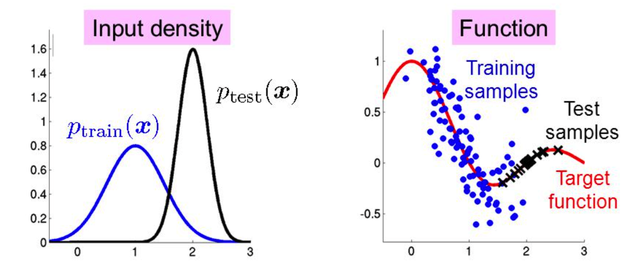
\includegraphics[width=9cm]{../assets/immagine.png}
		\label{fig:immagine}
	\end{figure}
\end{frame}

\begin{frame}{Inaccurate Model}
	\begin{figure}[H]
		\centering
		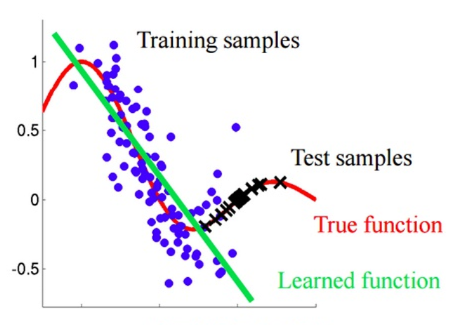
\includegraphics[width=6cm]{../assets/inacurate_model.png}
		\label{fig:inacurate_model}
	\end{figure}
	Changes in the features distribution can significantly impact the model's \textit{effectiveness}.
\end{frame}

\begin{frame}{Example}
	Consider a model designed to distinguish between images of cats and dogs:
	
	\vspace{0.5cm}
	\begin{minipage}[t]{0.55\textwidth} % 45% della larghezza per l'immagine
		\begin{flushleft}
			\textbf{\textcolor{blue}{Training set:}}
		\end{flushleft}
		\centering
		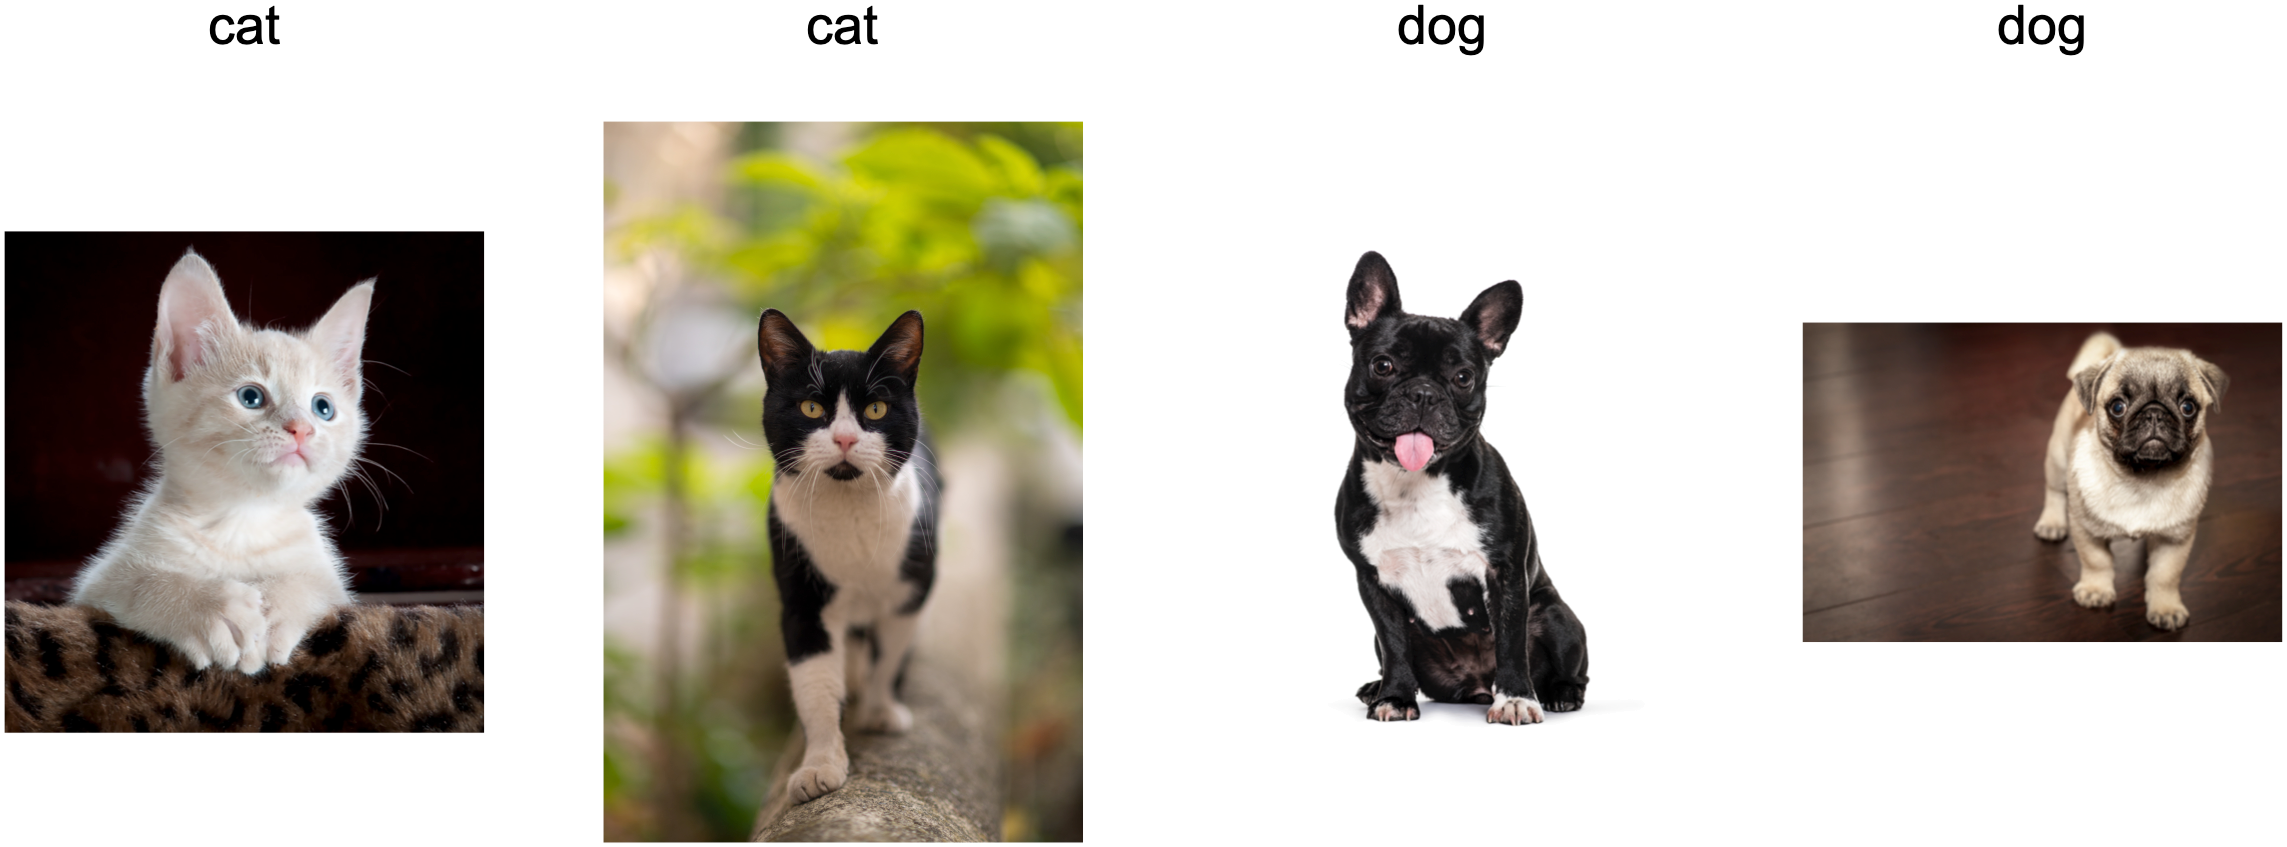
\includegraphics[width=5cm]{../assets/cat-dog-train.png}
		\label{fig:cani-gatti-train}
		\vspace{-0.2cm}
		\begin{flushleft}
			\textbf{\textcolor{blue}{Test set:}}
		\end{flushleft}
		\centering
		
\includegraphics[width=5cm]{../assets/cat-dog-test.png}
		\label{fig:cani-gatti-test}
		
	\end{minipage}
	\hfill
	\begin{minipage}[t]{0.35\textwidth} % 45% della larghezza per la didascalia
		\vspace{0.2cm}
		\begin{tcolorbox}[colframe=blue!50!black, colback=blue!5, coltitle=black, sharp corners]
			Model will not accurately distinguish between cats and dogs because the feature distribution will differ.
		\end{tcolorbox}
	\end{minipage}
\end{frame}


%  \end{document}